\documentclass{article}
\usepackage[utf8]{inputenc}
\usepackage{amsmath}
\usepackage{graphicx}
\usepackage[usepolish]{babel}
\usepackage{polski}
\usepackage[T1]{fontenc}
\usepackage{longtable}
\usepackage{pgfplots}


\title{latex - sprawozdanie}
\author{Piotr Strycharczyk}
\date{Grudzień 2022}

\begin{document}

\maketitle

\section{Wprowadzenie teoretyczne}
Spadek swobodny – ruch odbywający się wyłącznie pod wpływem ciężaru (siły grawitacji), bez oporów ośrodka.\\

\begin{equation}
h=h_0-g*t^2*1/2
\label{Równanie 1 spadku swobodnego}
\end{equation}\\
Równanie spadku swobodnego (\ref{Równanie 1 spadku swobodnego})


\section{Opis eksperymentu}

Eksperyment polega na upuszczeniu żelaznej kulki z pewnej wysokości h oraz zmierzeniu jej czasu spadku swobodnego. Jak widać na rysunku (\ref{zdjecie 1}) ciało spada swobodnie bez oporów.

\begin{figure}[htb]
    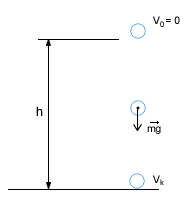
\includegraphics[width=6cm]{images.png}
    \centering
    \caption{przedstawia przebieg eksperymentu}
    \label{zdjecie 1}
\end{figure}


\section{Wyniki pomiarów}
Wynikami pomiarów jest tabelka (\ref{tabelka 1}) stu pomiarow czasu

\begin{longtable}{|l|l|l|}

\hline \multicolumn{1}{|c|}{\textbf{Lp.1}} & \multicolumn{1}{c|}{\textbf{t[s]}} & \multicolumn{1}{c|}{\textbf{s daszek}} \\ \hline 
\endfirsthead

\hline \multicolumn{1}{|c|}{\textbf{Lp.1}} & \multicolumn{1}{c|}{\textbf{t[s]}} & \multicolumn{1}{c|}{\textbf{s daszek}} \\ \hline 
\endhead



        1 & 0.10 & -0.12 \\ \hline
        2 & 0.20 & 0.28 \\ \hline
        3 & 0.30 & 0.41 \\ \hline
        4 & 0.40 & 0.79 \\ \hline
        5 & 0.50 & 1.21 \\ \hline
        6 & 0.60 & 1.73 \\ \hline
        7 & 0.70 & 2.44 \\ \hline
        8 & 0.80 & 3.15 \\ \hline
        9 & 0.90 & 4.05 \\ \hline
        10 & 1.00 & 4.80 \\ \hline
        11 & 1.10 & 5.92 \\ \hline
        12 & 1.20 & 7.12 \\ \hline
        13 & 1.30 & 8.13 \\ \hline
        14 & 1.40 & 9.40 \\ \hline
        15 & 1.50 & 11.02 \\ \hline
        16 & 1.60 & 12.51 \\ \hline
        17 & 1.70 & 14.19 \\ \hline
        18 & 1.80 & 15.87 \\ \hline
        19 & 1.90 & 17.56 \\ \hline
        20 & 2.00 & 19.65 \\ \hline
        21 & 2.10 & 21.65 \\ \hline
        22 & 2.20 & 23.59 \\ \hline
        23 & 2.30 & 26.07 \\ \hline
        24 & 2.40 & 28.18 \\ \hline
        25 & 2.50 & 30.74 \\ \hline
        26 & 2.60 & 33.21 \\ \hline
        27 & 2.70 & 35.66 \\ \hline
        28 & 2.80 & 38.41 \\ \hline
        29 & 2.90 & 41.25 \\ \hline
        30 & 3.00 & 44.09 \\ \hline
        31 & 3.10 & 47.03 \\ \hline
        32 & 3.20 & 50.06 \\ \hline
        33 & 3.30 & 53.24 \\ \hline
        34 & 3.40 & 56.50 \\ \hline
        35 & 3.50 & 59.98 \\ \hline
        36 & 3.60 & 63.66 \\ \hline
        37 & 3.70 & 67.07 \\ \hline
        38 & 3.80 & 70.77 \\ \hline
        39 & 3.90 & 74.58 \\ \hline
        40 & 4.00 & 78.42 \\ \hline
        41 & 4.10 & 82.49 \\ \hline
        42 & 4.20 & 86.45 \\ \hline
        43 & 4.30 & 90.65 \\ \hline
        44 & 4.40 & 94.84 \\ \hline
        45 & 4.50 & 99.34 \\ \hline
        46 & 4.60 & 103.54 \\ \hline
        47 & 4.70 & 108.17 \\ \hline
        48 & 4.80 & 112.88 \\ \hline
        49 & 4.90 & 117.66 \\ \hline
        50 & 5.00 & 122.58 \\ \hline
        51 & 5.10 & 127.51 \\ \hline
        52 & 5.20 & 132.39 \\ \hline
        53 & 5.30 & 137.63 \\ \hline
        54 & 5.40 & 142.69 \\ \hline
        55 & 5.50 & 148.29 \\ \hline
        56 & 5.60 & 153.68 \\ \hline
        57 & 5.70 & 159.34 \\ \hline
        58 & 5.80 & 164.87 \\ \hline
        59 & 5.90 & 170.48 \\ \hline
        60 & 6.00 & 176.57 \\ \hline
        61 & 6.10 & 182.27 \\ \hline
        62 & 6.20 & 188.39 \\ \hline
        63 & 6.30 & 194.41 \\ \hline
        64 & 6.40 & 200.84 \\ \hline
        65 & 6.50 & 207.02 \\ \hline
        66 & 6.60 & 213.32 \\ \hline
        67 & 6.70 & 220.05 \\ \hline
        68 & 6.80 & 226.44 \\ \hline
        69 & 6.90 & 233.32 \\ \hline
        70 & 7.00 & 240.00 \\ \hline
        71 & 7.10 & 247.05 \\ \hline
        72 & 7.20 & 253.90 \\ \hline
        73 & 7.30 & 261.03 \\ \hline
        74 & 7.40 & 268.19 \\ \hline
        75 & 7.50 & 275.61 \\ \hline
        76 & 7.60 & 283.23 \\ \hline
        77 & 7.70 & 290.58 \\ \hline
        78 & 7.80 & 298.18 \\ \hline
        79 & 7.90 & 305.85 \\ \hline
        80 & 8.00 & 313.77 \\ \hline
        81 & 8.10 & 321.28 \\ \hline
        82 & 8.20 & 329.51 \\ \hline
        83 & 8.30 & 337.71 \\ \hline
        84 & 8.40 & 345.93 \\ \hline
        85 & 8.50 & 353.98 \\ \hline
        86 & 8.60 & 362.37 \\ \hline
        87 & 8.70 & 370.86 \\ \hline
        88 & 8.80 & 379.41 \\ \hline
        89 & 8.90 & 388.12 \\ \hline
        90 & 9.00 & 396.90 \\ \hline
        91 & 9.10 & 405.83 \\ \hline
        92 & 9.20 & 415.00 \\ \hline
        93 & 9.30 & 423.69 \\ \hline
        94 & 9.40 & 432.87 \\ \hline
        95 & 9.50 & 442.40 \\ \hline
        96 & 9.60 & 451.39 \\ \hline
        97 & 9.70 & 461.08 \\ \hline
        98 & 9.80 & 470.30 \\ \hline
        99 & 9.90 & 480.36 \\ \hline
        100 & 10.00 & 490.06 \\ \hline
\caption{Wyniki pomiarów}
\label{tabelka 1}
\end{longtable}

\begin{tikzpicture}
\begin{axis}[
    title={Wykres spadku swobodnego},
    xmin=0, xmax=10,
    ymin=0, ymax=600,
    xtick={0,1,2,3,4,5,6,7,8,9,10},
    ytick={0,100,200,300,400,500,600},
    axis lines = left,
    xlabel = \(czas(t)\),
    ylabel = \(droga(m)\),
    domain=0:10,
]
%Below the red parabola is defined
\addplot [ 
    color=blue,
    ultra thick,
]
{4.9*x^2 };

\addplot [ 
color=orange,
only marks,
mark=square,
mark size=0.4pt]
table[meta=t]
{csv5.csv};

 
\addlegendentry{\(g*t^2*1/2\)}

\end{axis}
\end{tikzpicture}

\section{Wnioski}
Gdy ciało spada z większej wysokości to przy ziemi osiąga większą prędkość.

\end{document}
